\chapter{Iteración 5}

\begin{quotation}[Computer Scientist]{Harold Abelson (1947--)}
Programs must be written for people to read, and only incidentally for machines to execute.
\end{quotation}

\begin{abstract}
Esta iteración se centra en el núcleo jugable del combate. En ella se actualiza la
presentación visual del jugador y se incorporan los sistemas de combate y de enemigos que
permiten definir interacciones ofensivas, tipos de comportamiento y respuesta al daño.
\end{abstract}

\section{Análisis de características}
La quinta iteración se centró en reforzar la identidad jugable del proyecto a través del
combate, del comportamiento enemigo y de la presentación visual del personaje. Hasta este
punto, el sistema ya permitía explorar, progresar por círculos, alternar entre formas y
orientarse dentro del mapa, pero la sensación jugable seguía dependiendo en gran medida de
la solidez del combate y de la respuesta de los enemigos. Por ello, esta iteración se
articula en torno a tres funcionalidades: el ajuste de sprites del jugador, la ampliación
del sistema de combate y la consolidación del sistema de enemigos.

\begin{enumerate}
\item \textbf{Actualizar Sprites.} Esta funcionalidad se centró en refinar la presentación
animada del personaje, ajustando la cadencia de reproducción de los sprites para que su
movimiento y sus distintas formas resultaran más coherentes visualmente. El trabajo
realizado en esta iteración no consistió en sustituir por completo los recursos gráficos,
sino en corregir su ritmo de reproducción para que la percepción del desplazamiento y de la
animación no fuera excesivamente rápida o inconsistente entre variantes. En términos
funcionales, esta feature mejora la lectura del personaje en pantalla y acompaña mejor la
respuesta del sistema de control, lo que resulta especialmente importante en un juego donde
la claridad visual afecta directamente a la sensación de precisión. Aunque se trata de una
mejora menos estructural que otras features de esta iteración, su impacto sobre la calidad
percibida del movimiento del jugador es significativo.

\begin{figure}[H]
\begin{center}
\missingfigure{Sustituir por captura representativa de Actualizar Sprites en la iteración 5}
% \includegraphics[width=.9\textwidth]{figures/iteracion5_actualizar_sprites.png}
\caption{Resultado visual de la feature Actualizar Sprites en la iteración 5}
\label{fig:iteracion5-feature-sprites}
\end{center}
\end{figure}

\item \textbf{Sistema de combate.} Esta funcionalidad amplió de forma sustancial el combate
del jugador para adaptarlo a distintas armas y a las dos formas ya introducidas en la
dualidad de personajes. Su funcionamiento real dejó de depender de un único ataque
genérico y pasó a organizarse alrededor de definiciones de arma con comportamiento propio.
Esto permitió distinguir entre ataques de melé y ataques de proyectil, gestionar tiempos de
reutilización independientes, definir alcances distintos y soportar ataques cargados en las
armas que lo requieren. Además, el sistema pasó a registrar el contexto del daño generado,
incluyendo el arma utilizada y la forma activa del jugador, lo que prepara el terreno para
interacciones más ricas con el comportamiento enemigo. En la práctica, esta feature hizo que
el combate dejara de ser una acción uniforme y pasara a responder a la identidad de cada
arma y a la forma actual del personaje, aumentando la profundidad táctica de la partida.

\begin{figure}[H]
\begin{center}
\missingfigure{Sustituir por captura representativa del Sistema de combate en la iteración 5}
% \includegraphics[width=.9\textwidth]{figures/iteracion5_sistema_combate.png}
\caption{Resultado visual de la feature Sistema de combate en la iteración 5}
\label{fig:iteracion5-feature-combate}
\end{center}
\end{figure}

\item \textbf{Sistema de enemigos.} Esta funcionalidad consolidó el comportamiento enemigo
para hacerlo más compatible con el nuevo sistema de combate y con la variedad creciente del
juego. Su alcance real no se limitó a corregir errores de aparición en salas, sino que
extendió la lógica de los enemigos con comportamientos diferenciados por tipo, integración
con proyectiles enemigos y una respuesta más rica al daño recibido según el arma utilizada.
La feature mejoró además el proceso de aparición y activación de enemigos dentro de las
habitaciones, apoyándose en zonas de spawn ponderadas y en una mejor coordinación con el
estado de la sala. A esto se suma la incorporación de ataques a distancia para determinados
enemigos y la introducción de multiplicadores de daño dependientes del contexto del arma y
del tipo de enemigo. En conjunto, esta funcionalidad convirtió a los enemigos en agentes
más variados y mejor integrados con el resto del combate, haciendo que la oposición del
juego se sintiera menos genérica y más conectada con las decisiones del jugador.

\begin{figure}[H]
\begin{center}
\missingfigure{Sustituir por captura representativa del Sistema de enemigos en la iteración 5}
% \includegraphics[width=.9\textwidth]{figures/iteracion5_sistema_enemigos.png}
\caption{Resultado visual de la feature Sistema de enemigos en la iteración 5}
\label{fig:iteracion5-feature-enemigos}
\end{center}
\end{figure}
\end{enumerate}

La combinación de estas tres funcionalidades convirtió la quinta iteración en una fase
claramente orientada a la jugabilidad. Más que añadir nuevas capas de planificación o de
interfaz, esta entrega reforzó el núcleo de acción del videojuego, mejorando tanto la
respuesta del jugador como la calidad de la oposición que ofrece el sistema.

\section{Diseño}
El diseño de esta iteración partió de una necesidad evidente: si el combate debía ser uno
de los pilares centrales de \textit{Via Inferni}, no podía seguir apoyándose en un modelo
demasiado uniforme ni en enemigos con comportamientos poco diferenciados. El objetivo fue
dotar tanto al jugador como a sus adversarios de una lógica más expresiva sin perder el
control sobre la modularidad del sistema.

\subsection{Diseño de la actualización visual del jugador}
El ajuste de sprites se planteó como un refinamiento de percepción más que como una
reestructuración profunda. La decisión importante aquí fue reconocer que la calidad del
movimiento no depende únicamente de la entrada y del desplazamiento físico, sino también del
ritmo con el que las animaciones se reproducen en pantalla.

Por ello, el diseño de esta mejora se centró en el control de la velocidad de reproducción
de las secuencias de sprites, buscando una sensación visual más coherente entre las
distintas variantes del personaje.

\subsection{Diseño del sistema de combate}
La decisión central de esta feature fue diseñar el combate en torno a definiciones de arma,
en lugar de codificar comportamientos específicos de forma rígida dentro del controlador del
jugador. Esto permite que cada arma disponga de identidad propia mediante parámetros como
daño base, \textit{cooldown}, alcance, tipo de ataque, proyectil, comportamiento de carga o
retroceso aplicado al objetivo.

Además, se decidió que el combate debía integrarse con la dualidad de formas ya existente.
Por ello, el sistema se organizó en pools de armas de melé y a distancia, seleccionadas en
función de la forma actual del jugador. También se tuvo en cuenta la necesidad de conservar
el contexto del daño producido, ya que esto permite que otras entidades, como los enemigos,
interpreten de forma distinta un mismo impacto según el arma o la forma que lo originan.

\subsection{Diseño del sistema de enemigos}
El rediseño de enemigos se apoyó en dos líneas principales. La primera fue diferenciar su
comportamiento por tipo, de forma que no todos compartieran la misma respuesta táctica. La
segunda fue conectarlos de manera más estrecha con el nuevo combate del jugador.

Esto llevó a definir enemigos con patrones distintos, como aproximación directa, gestión de
distancia o ataques proyectados, y a permitir que la recepción del daño dependa también del
arma empleada. De este modo, el sistema de enemigos deja de ser un simple conjunto de
objetivos que persiguen al jugador y pasa a formar parte de una relación táctica más rica.

\section{Implementación}
La implementación de esta iteración se repartió entre ajustes sobre la capa visual del
jugador, ampliación del subsistema de combate y refuerzo del comportamiento enemigo. A
medida que el proyecto gana complejidad, estas tres áreas empiezan a funcionar cada vez más
como partes de un mismo bloque jugable.

\subsection{Implementación de Actualizar Sprites}
La mejora visual del jugador se materializó mediante un ajuste en el componente
\texttt{PlayerSpriteAnimator}, reduciendo o equilibrando los fotogramas por segundo usados
por las distintas variantes visuales del personaje. El cambio se aplicó sobre la
configuración del prefab del jugador, sin necesidad de reescribir la lógica general del
animador.

Aunque la implementación es pequeña en comparación con otras features de la iteración, su
efecto práctico es claro: la animación deja de percibirse con una cadencia poco natural y
se integra mejor con la velocidad real de movimiento del personaje.

\subsection{Implementación del sistema de combate}
La ampliación del combate se apoyó principalmente en \texttt{PlayerCombatController},
\texttt{WeaponDefinition}, \texttt{MeleeHitbox} y \texttt{Projectile}. El controlador de
combate pasó a resolver los ataques a partir del arma actualmente seleccionada, consultando
si se trata de un ataque de melé o de proyectil y aplicando la lógica correspondiente.

En el caso de la melé, el sistema genera una hitbox temporal asociada al jugador, capaz de
infligir daño, evitar autocolisiones y aplicar empuje cuando el arma así lo requiere. En el
caso de los proyectiles, se instancia un objeto con velocidad, vida útil y, en algunos
casos, capacidad de guiado hacia objetivos válidos. También se añadió soporte para ataques
cargados, donde el daño final depende del tiempo de preparación acumulado.

Una pieza importante de esta implementación es \texttt{DamageSourceContext}, que conserva el
origen del daño, el identificador del arma y la forma del jugador. Esto permite que el daño
no llegue al objetivo como un valor aislado, sino acompañado de contexto útil para otros
sistemas.

\subsection{Implementación del sistema de enemigos}
La consolidación del sistema de enemigos se apoyó en cambios sobre \texttt{EnemyController},
\texttt{EnemyProjectile} y \texttt{Room}. En primer lugar, los enemigos pasaron a incorporar
comportamientos diferenciados según su tipo, ajustando persecución, distancia preferida,
ataque cuerpo a cuerpo o ataque a distancia.

En segundo lugar, se integró un proyectil específico para enemigos, permitiendo que
determinadas variantes, como las voladoras, pudieran dañar al jugador sin depender
exclusivamente del contacto directo. En tercer lugar, se reforzó la relación entre sala y
enemigos durante el spawn, la activación al entrar por primera vez y el desbloqueo de
puertas cuando el encuentro termina.

Por último, los enemigos pasaron a interpretar el contexto del arma que les daña,
modificando el multiplicador de daño según su tipo y según la herramienta utilizada por el
jugador. Esto conecta directamente el comportamiento enemigo con la variedad introducida por
el nuevo sistema de combate.

\section{Seguimiento y control}
El seguimiento de esta iteración permitió comprobar que el núcleo del combate podía quedar
operativo dentro del tiempo previsto, pero también puso de manifiesto que tanto el sistema de
combate como el sistema de enemigos tenían más recorrido del estimado inicialmente. La
iteración cerró una base funcional sólida, con armas diferenciadas, proyectiles y enemigos
mejor integrados, pero durante el desarrollo se vio que aún quedaban aspectos de legibilidad,
\textit{feedback} y diferenciación táctica que no convenía forzar en el mismo ciclo.

Desde el punto de vista temporal, la iteración quedó incluso ligeramente por debajo de la
estimación: frente a las 50:00 horas planificadas, se registraron 48:22 horas reales. Esto
significa que el ajuste no vino dado por una falta inmediata de tiempo, sino por una mejor
comprensión del alcance real de las features a medida que se desarrollaban.

Por ello, el control del avance llevó a considerar combate y enemigos como sistemas cerrados
en una primera fase, pero no completamente agotados. Su refinamiento posterior se
replanificó para la iteración 7. Esta decisión encaja con la observación general del
proyecto: algunas features se habían estimado inicialmente como menos complejas de lo que
realmente fueron, y dividirlas entre iteraciones permitió ajustar mejor el esfuerzo al
resultado esperado.

\begin{table}[h!]
    \centering
    \begin{coolTable}{lr}{2}
    {Horas de la iteración 5}
    \textbf{Horas planificadas de la iteración} & 50:00 \\
    \textbf{Horas reales (Adolfo Borrego González)} & 22:48 \\
    \textbf{Horas reales (Germán Sánchez Carmona)} & 25:34 \\
    \textbf{Horas reales totales de la iteración} & 48:22 \\
    \textbf{Horas acumuladas planificadas hasta esta iteración} & 350:00 \\
    \textbf{Horas acumuladas reales hasta esta iteración} & 351:52 \\
    \end{coolTable}
    \caption{Resumen de horas reales de la iteración 5.}
\end{table}

\begin{figure}[htbp]
\begin{center}
% \missingfigure{Sustituir por el diagrama UML de resultado de la iteración 5}
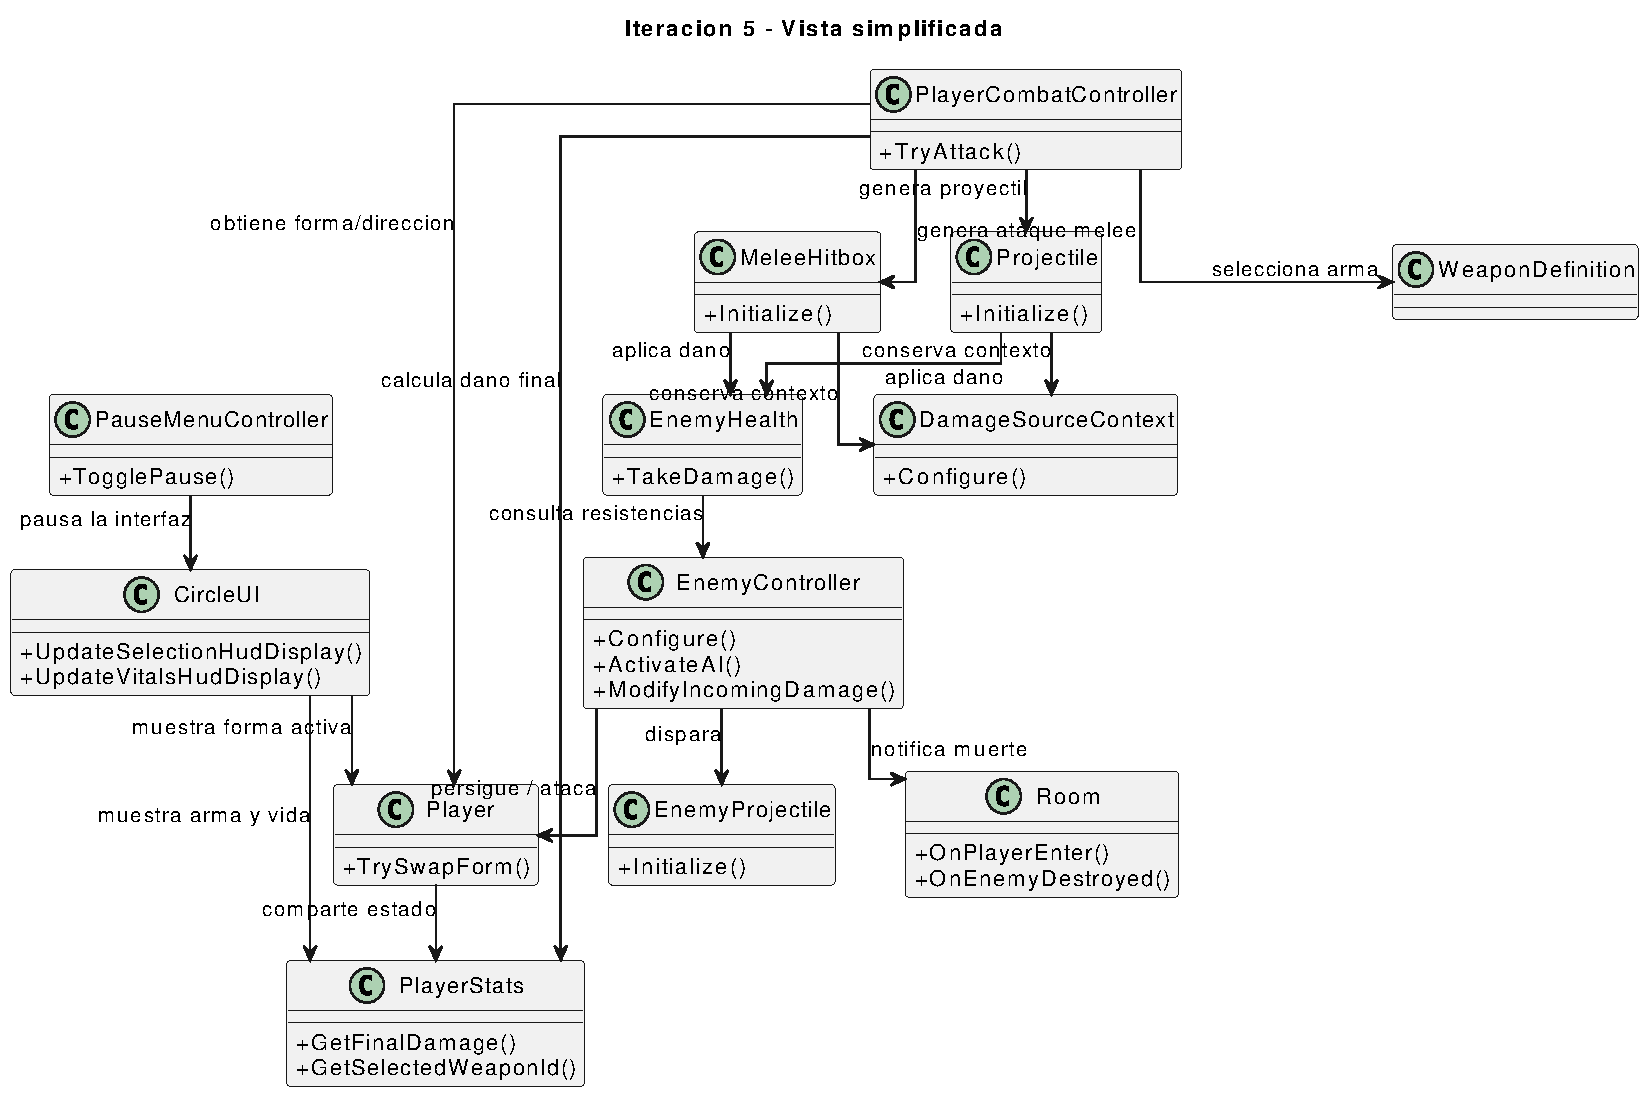
\includegraphics[width=\textwidth]{figures/iteracion5_resultado_uml.pdf}
\caption{Diagrama UML de resultado de la iteración 5}
\label{fig:uml-resultado-iteracion5}
\end{center}
\end{figure}
